\section{Numerical Results}\label{sec:results}

\subsection{Setup}
Unless otherwise stated, the parameters of Table~\ref{tab:params} are used with $M=128$ STAR-RIS elements (reduced from 256 for tractable runtime), a $16\times16$ satellite UPA, Rician factor $\kappa=10$\,dB on the satellite link, and a GNSS-class spoofer with $P_a=-10$\,dBm located 40\,m from the STAR-RIS in the reflection half-space; the spoofing interference reaches each user over a 50\,m ground link. Artificial noise consumes 20\% of the power budget isotropically. The proposed algorithm is initialized from three candidate points (random, conventional-RIS warm start, and continuation from the previous power point) and the best converged solution is retained; this is legitimate since the STAR-RIS design subsumes the reflecting-only design as a special case.

\subsection{Sum Secrecy Rate}
Fig.~\ref{fig:secrecy} compares the sum secrecy rate versus the satellite transmit power for four schemes: (i) the proposed STAR-RIS near-field ISAC design, (ii) a conventional reflection-only RIS (transmission-side users unserved), (iii) a random-phase STAR-RIS with MRT, and (iv) a blocked direct link without RIS (30\,dB shadowing). Since all schemes solve non-convex problems, each curve reports the best result obtained over multiple initializations (random, warm-start, and continuation over $P_{\max}$). The proposed design matches or outperforms all benchmarks at every power point, with the gap widening at high power (17.0 vs.\ 16.1\,bps/Hz for the conventional RIS at $P_{\max}=45$\,dBm), where the STAR-RIS's full-space coverage simultaneously serves both half-spaces while suppressing the leakage toward the spoofer. The random-phase STAR-RIS achieves almost zero secrecy rate, confirming that the cascaded LEO--RIS--user link is unusable without proper phase design, and the no-RIS scheme is limited by the blocked direct link.

\subsection{Convergence}
Fig.~\ref{fig:conv} shows the convergence of the proposed AO algorithm (with the monotone acceptance guard) from a random-phase initialization: the sum secrecy rate rises from near zero to its converged value within the first outer iteration and remains stable thereafter, validating the low-complexity nature of the design with the proposed warm-start strategy.

\subsection{Localization Accuracy (CRB) and Tracking}
Fig.~\ref{fig:crb} depicts the Cram\'er--Rao bound of the spoofer's range estimate versus its distance from the STAR-RIS, using a monostatic anchor with 10\,W sensing power and the two-way echo path loss. The near-field spherical-wave model yields a sub-meter-level ranging accuracy ($\sqrt{\mathrm{CRB}_r} \approx 0.84$\,m at 50\,m, i.e., $\mathrm{CRB}_r \approx 0.7\,\mathrm{m}^2$, below the threshold $\epsilon_{\mathrm{CRB}}=1\,\mathrm{m}^2$ of Table~\ref{tab:params}), while the far-field (planar-wave) approximation yields a singular FIM --- the range is fundamentally unobservable, shown capped at $10^3$\,m. This quantifies the key sensing advantage that the proposed framework exploits. Feeding such range/angle measurements into the EKF of Section~\ref{sec:sensing} gives a spoofer tracking RMSE of $\approx 0.36$\,m over a 30\,s trajectory (Fig.~\ref{fig:ekf}), which is sufficiently accurate for reconstructing the wiretap channel $\mathbf{h}_a$ used in the beamforming design.

\begin{figure}[t]
\centering
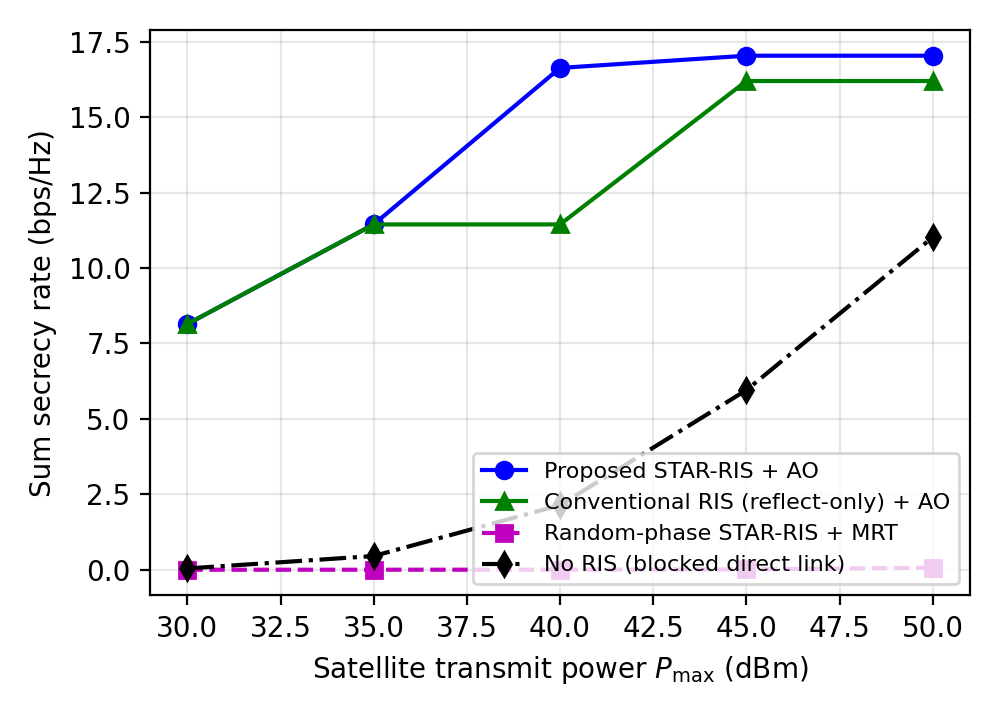
\includegraphics[width=\columnwidth]{figs/fig_secrecy_vs_pmax.png}
\caption{Sum secrecy rate vs.\ satellite transmit power: proposed STAR-RIS near-field ISAC vs.\ benchmarks.}
\label{fig:secrecy}
\end{figure}

\begin{figure}[t]
\centering
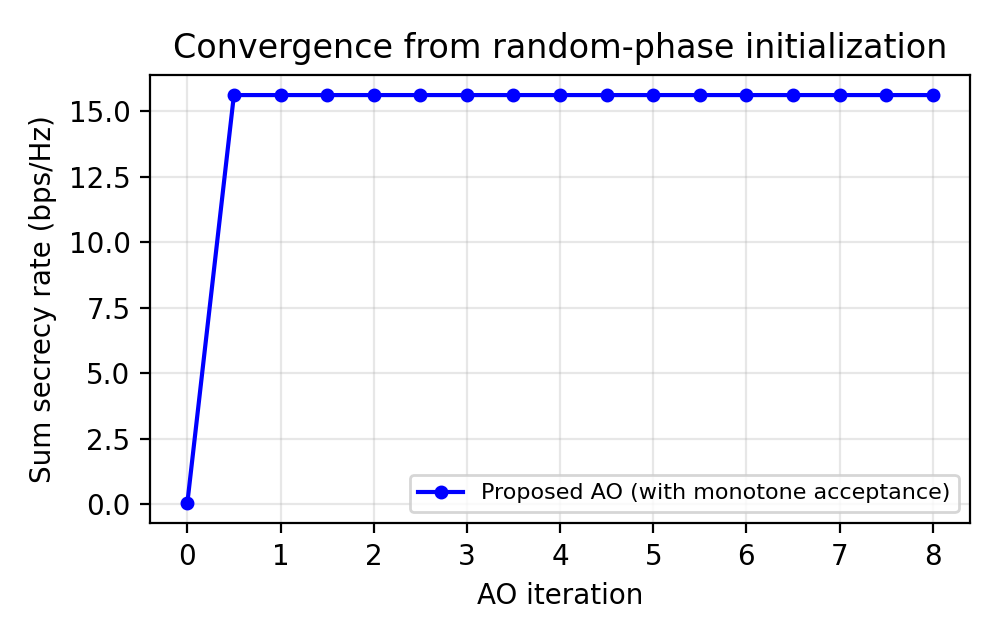
\includegraphics[width=\columnwidth]{figs/fig_convergence.png}
\caption{Convergence of the proposed AO algorithm ($P_{\max}=50$\,dBm).}
\label{fig:conv}
\end{figure}

\begin{figure}[t]
\centering
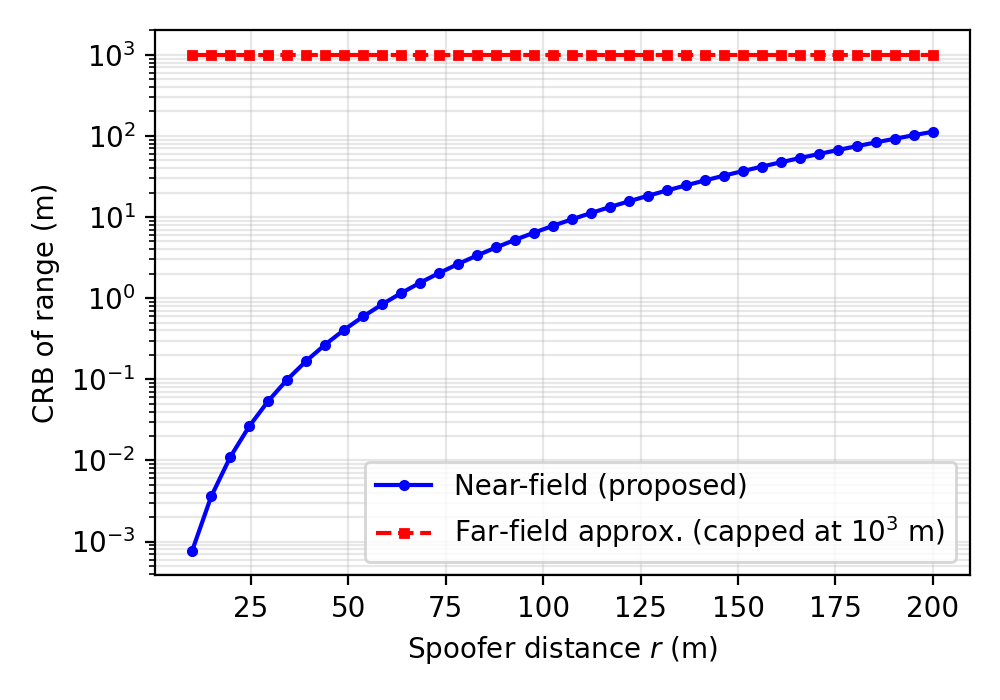
\includegraphics[width=\columnwidth]{figs/fig_crb.png}
\caption{CRB of the spoofer range estimate: near-field vs.\ far-field model.}
\label{fig:crb}
\end{figure}

\subsection{Robustness to Spoofer Localization Error}
Since the beamforming design relies on the spoofer channel \emph{reconstructed} from the sensed position (Remark~1), Fig.~\ref{fig:robust} evaluates the achieved sum secrecy rate when the true spoofer position deviates from the estimate by a random error of standard deviation $\sigma_e$ (60 Monte-Carlo realizations per level, fixed design). Two observations are made. First, at the accuracy actually delivered by the EKF ($\sigma_e \approx 0.36$\,m), the worst-case degradation over all realizations is only $4.5\%$ ($10.33$ vs.\ $10.81$\,bps/Hz), confirming that the ISAC sensing accuracy is sufficient for the secrecy design. Second, the mean achieved rate slightly \emph{increases} with $\sigma_e$: in this geometry the spoofer's nominal direction is nearly aligned with one user's near-field channel (the worst case, which the design suppresses at some rate sacrifice), so a position mismatch only decouples the spoofer from that user; the achieved rate never falls more than $4.5\%$ below the design value even at $\sigma_e=4$\,m, roughly seven times the array's transverse near-field resolution ($\approx 0.6$\,m at 40\,m).

\begin{figure}[t]
\centering
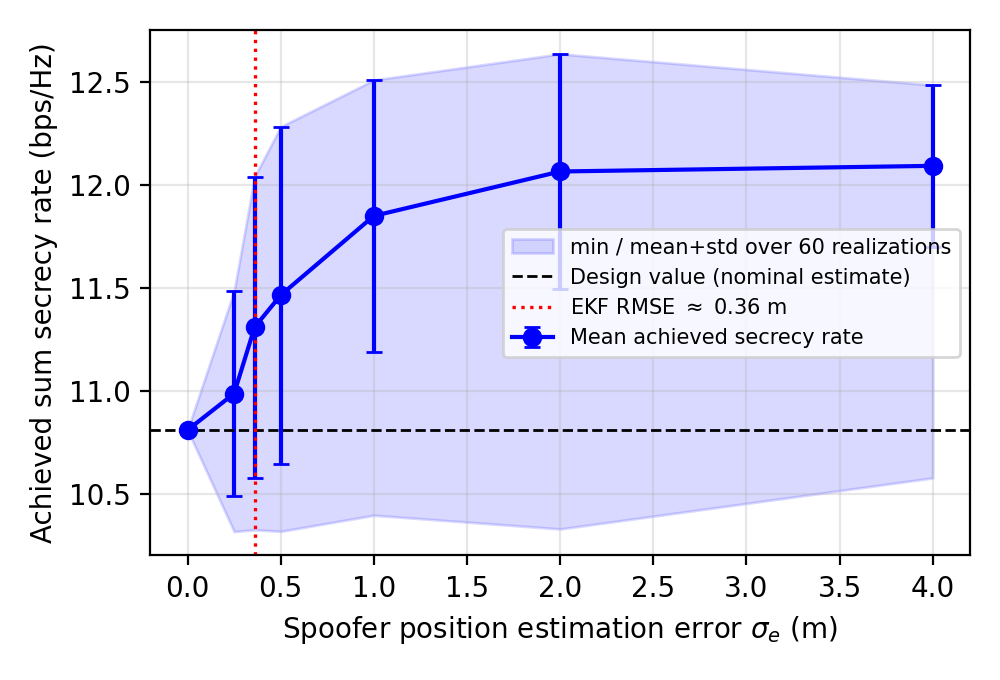
\includegraphics[width=\columnwidth]{figs/fig_robustness.png}
\caption{Achieved sum secrecy rate vs.\ spoofer-position estimation error (60 Monte-Carlo realizations; shaded: min to mean+std).}
\label{fig:robust}
\end{figure}

\begin{figure}[t]
\centering
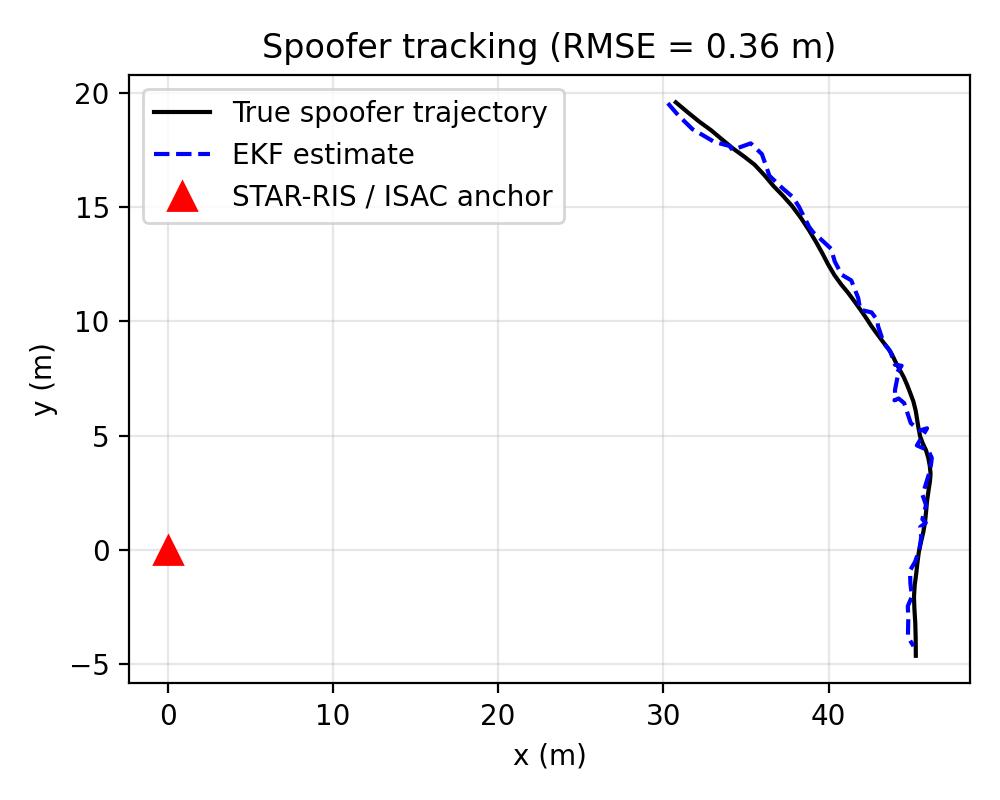
\includegraphics[width=\columnwidth]{figs/fig_ekf.png}
\caption{EKF-based spoofer trajectory tracking (position RMSE $\approx 0.36$\,m).}
\label{fig:ekf}
\end{figure}
